\section{Laboratory work implementation}

\subsection{Tasks and Points}

Basic Level:

    - Draw 5 lines
    
    - Draw 5 bezier curves
   
    - Draw 4 plane objects
    
    - Draw 2 objects using mouse


Normal Level:

    - Realize the tasks from Basic Level.

    - Custom bitmap
    
    - Fill 2 objects with gradient


Advanced Level:

	- Use mouse as eraser

\subsection{Laboratory work analysis}

Repository:

https://github.com/VictorIstratii151/WP-labs

\subsection{Proving my work}

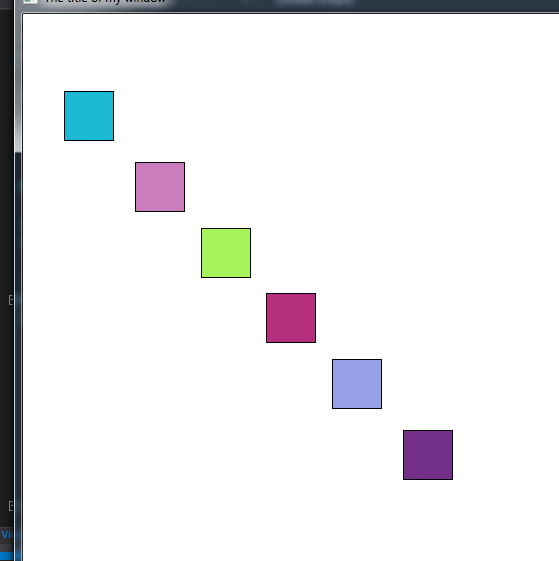
\includegraphics{im1}
From start you can observe that my application has a custom bitmap as background



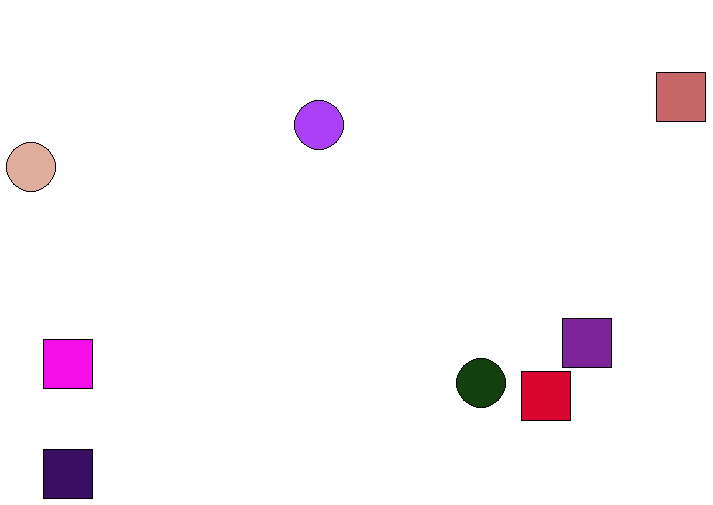
\includegraphics{im2}
From drop-down menu we can draw  random lines of random weight and colour



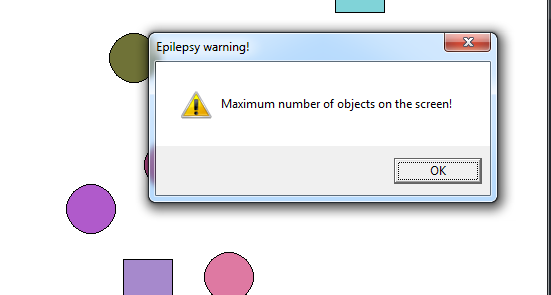
\includegraphics{im3}
From drop-down menu also can be drawn 4 plane objects

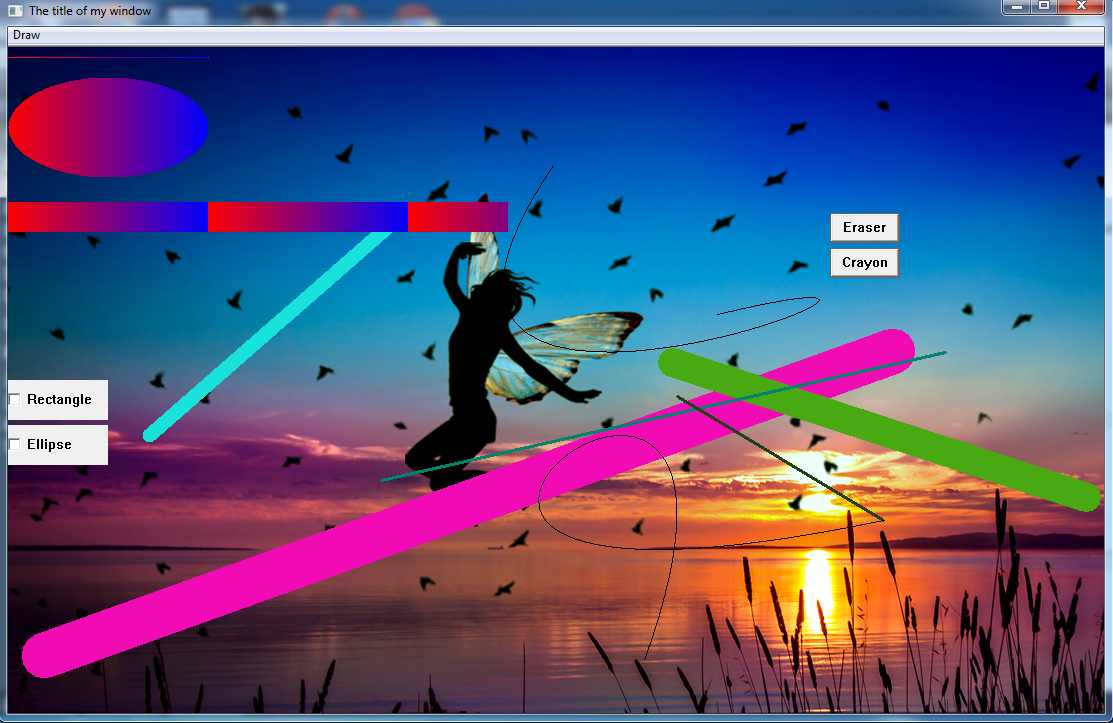
\includegraphics{im4}
From drop-down menu we can draw 2 bezier curves too


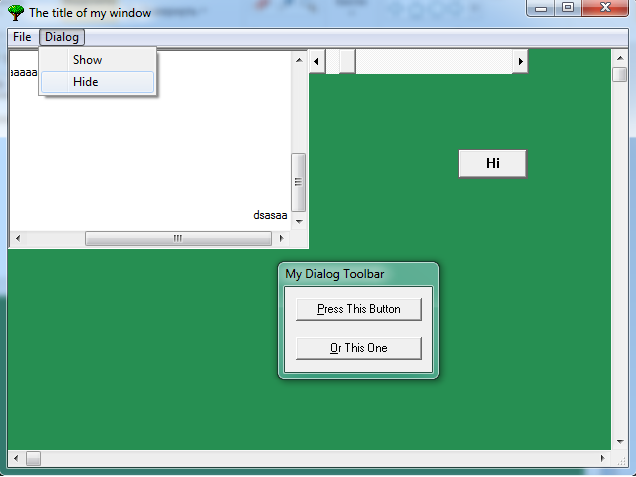
\includegraphics{im6}
You can see here how on the background are drawn several objects filled with gradient. They Are static. I have highlighted them with a red shape. To choose the red crayon I just simply click on the  button representing it. 




\includegraphics{im7}
The eraser has the same principle of working as the crayon. But we need to consider disabling the crayon first, before using the eraser.

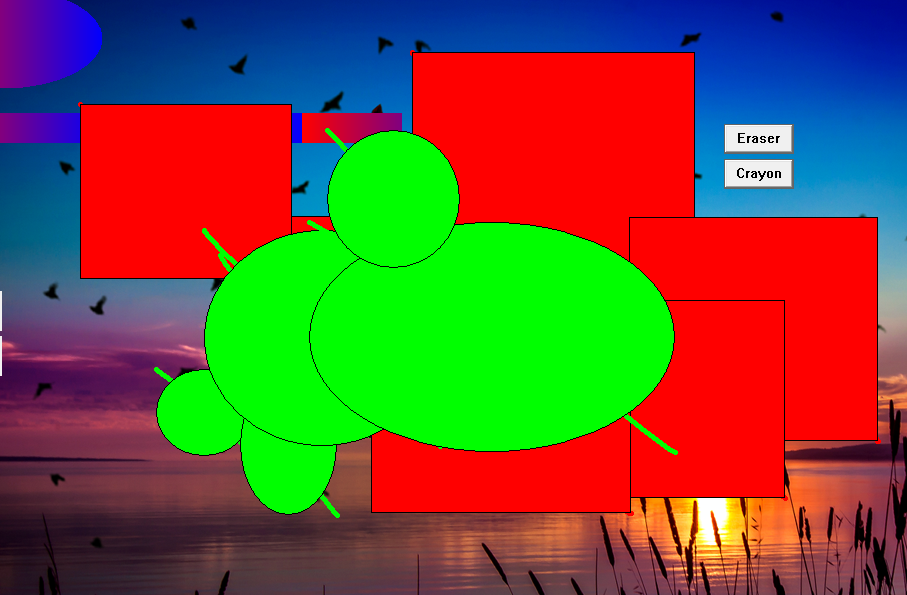
\includegraphics{im8}
On this screen you can see how we can draw shapes like ellipses or rectangles on the screen. To do this, the respective checkbox must be checked and the crayon must be enabled.


\clearpage